%%%%%%%%%%%%%%%%%%%%%%%%%%%%%%%%%%%%%%%%%%%%%%%%%%%%%%%%%%%%%%%%%%%%%%%%
%     LaTeX source code to approximate a NIST Technical report
%	  Instructions for authors: tinyurl.com/techpubsnist
%	DOI watermark will be added on final PDF
% 	Developed by K. Miller, kmm5@nist.gov
%	Last updated: 10-Oct-2017
%%%%%%%%%%%%%%%%%%%%%%%%%%%%%%%%%%%%%%%%%%%%%%%%%%%%%%%%%%%%%%%%%%%
\documentclass[12pt]{article}
\usepackage{adjustbox}
\usepackage{amsmath}
\usepackage{amsfonts}   % if you want the fonts
\usepackage{amssymb}    % if you want extra symbols
\usepackage{graphicx}   % need for figures
\usepackage{xcolor}
\usepackage{bm}
\usepackage{secdot}		
\usepackage{mathptmx}
\usepackage{multicol}
\usepackage{float}
\usepackage[utf8]{inputenc}
\usepackage{textgreek}
\usepackage{textcomp}
\usepackage[hang,flushmargin,bottom]{footmisc} % footnote format
\usepackage{rotating}
\usepackage{tikz}
\usepackage{siunitx} % Formats the units and values
\usepackage{titlesec}
\usepackage{tikz}
\titleformat{\section}{\normalsize\bfseries}{\thesection.}{1em}{}	% required for heading numbering style
\titleformat*{\subsection}{\normalsize\bfseries}

\usepackage{tocloft}	% change typeset, titles, and format list of appendices/figures/tables
\renewcommand{\cftdot}{}	
\renewcommand{\contentsname}{Table of Contents}
\renewcommand{\cftpartleader}{\cftdotfill{\cftdotsep}} % for parts
\renewcommand{\cftsecleader}{\cftdotfill{\cftdotsep}}
\renewcommand\cftbeforesecskip{\setlength{4pt}{}}
\addtolength{\cftfignumwidth}{1em}
\renewcommand{\cftfigpresnum}{\figurename\ }
\addtolength{\cfttabnumwidth}{1em}
\renewcommand{\cfttabpresnum}{\tablename\ }
\setlength{\cfttabindent}{0in}    %% adjust as you like
\setlength{\cftfigindent}{0in}

\usepackage{enumitem}         % to control spacing between bullets/numbered lists

\usepackage[numbers,sort&compress]{natbib} % format bibliography
\renewcommand{\bibsection}{}
\setlength{\bibsep}{0.0pt}

\usepackage[hidelinks]{hyperref} % hyperref package & removing outline from links

\usepackage{epstopdf} % converting EPS figure files to PDF

\usepackage{fancyhdr, lastpage}	% formatting document, calculating number of pages, formatting headers
\setlength{\topmargin}{-0.5in}
\setlength{\headheight}{39pt}
\setlength{\oddsidemargin}{0.25in}
\setlength{\evensidemargin}{0.25in}
\setlength{\textwidth}{6.0in}
\setlength{\textheight}{8.5in}

\usepackage{caption} % required for Figure labels
\captionsetup{font=small,labelfont=bf,figurename=Fig.,labelsep=period,justification=raggedright}

%%%%%%%%%%% !!!!!! REQUIRED - FILL OUT METADATA HERE !!!!!!!! %%%%%%%%%%%%%%
%  	Report Number - fill in Report Number sent to you (see info below)
%   DOI Statement - fill in DOI sent to you
%   Month Year - fill in Month and Year of Publication
%%%%%%%%%%%%%%%%%%%%%%%%%%%%%%%%%%%%%%%%%%%%%%%%%%%%%%%%%%%%%%%%%%%%%%%%%%%%%%%%%%%%%%
\newcommand{\pubnumber}{XXXX}
\newcommand{\DOI}{https://doi.org/10.6028/NIST.TN.XXXX}
\newcommand{\monthyear}{Month Year}
%%%%%%%%%%%%%%%%%%%%%%%%%%%%%%%%%%%%%%%%%%%%%%%%%%%%%%%%%%%%%%%%%%%%
%   	BEGIN DOCUMENT
%%%%%%%%%%%%%%%%%%%%%%%%%%%%%%%%%%%%%%%%%%%%%%%%%%%%%%%%%%%%%%%%%%%%
\begin{document}
	\urlstyle{rm} % Format style of \url
	
%%%%%%%%%%%%%%%%%%%%%%%%%%%%%%%%%%%%%%%%%%%%%%%%%%%%%%%%%%%%%%%%%%%%
%   Cover Page is REQUIRED and must contain the information
%	displayed here, at a minimum. Additional artwork may be included
%	(e.g., official project/conference logo, etc.).
%	Pub Number automated based on metadata
%%%%%%%%%%%%%%%%%%%%%%%%%%%%%%%%%%%%%%%%%%%%%%%%%%%%%%%%%%%%%%%%%%%%
	\begin{titlepage}
		\begin{flushright}
%%%%%%%%%%%%%%%%%%%%%%%%%%%%%%%%%%%%%%%%%%%%%%%%%%%%%%%%%%%%%%%%%%%%
% 	Automated based on metadata - delete if not applicable
%%%%%%%%%%%%%%%%%%%%%%%%%%%%%%%%%%%%%%%%%%%%%%%%%%%%%%%%%%%%%%%%%%%%
\LARGE{\textbf{NIST Technical Note \pubnumber}}\\
\vfill
%%%%%%%%%%%%%%%%%%%%%%%%%%%%%%%%%%%%%%%%%%%%%%%%%%%%%%%%%%%%%%%%%%%%
%	Title
%%%%%%%%%%%%%%%%%%%%%%%%%%%%%%%%%%%%%%%%%%%%%%%%%%%%%%%%%%%%%%%%%%%%
\Huge{\textbf{Measurement of the Flow Resistance of Vegetation}}\\
\vfill
%%%%%%%%%%%%%%%%%%%%%%%%%%%%%%%%%%%%%%%%%%%%%%%%%%%%%%%%%%%%%%%%%%%%
%	Authors - add complete list of authors, affiliations will be
%   added on title page
%%%%%%%%%%%%%%%%%%%%%%%%%%%%%%%%%%%%%%%%%%%%%%%%%%%%%%%%%%%%%%%%%%%%
\large Ryan Falkenstein-Smith\\
\large Kevin McGrattan\\
\large Marco Fernandez \\
\vfill
%%%%%%%%%%%%%%%%%%%%%%%%%%%%%%%%%%%%%%%%%%%%%%%%%%%%%%%%%%%%%%%%%%%%
%	The DOI is automated based on metadata.	
%%%%%%%%%%%%%%%%%%%%%%%%%%%%%%%%%%%%%%%%%%%%%%%%%%%%%%%%%%%%%%%%%%%%
\normalsize This publication is available free of charge from:\\
\DOI\\
\vfill
%%%%%%%%%%%%%%%%%%%%%%%%%%%%%%%%%%%%%%%%%%%%%%%%%%%%%%%%%%%%%%%%%%%%
%	NIST LOGO - keep as-is
%%%%%%%%%%%%%%%%%%%%%%%%%%%%%%%%%%%%%%%%%%%%%%%%%%%%%%%%%%%%%%%%%%%%


\includegraphics[width=0.3\linewidth]{NIST-logo.eps}\\


\end{flushright}
\end{titlepage}
\begin{titlepage}
%%%%%%%%%%%%%%%%%%%%%%%%%%%%%%%%%%%%%%%%%%%%%%%%%%%%%%%%%%%%%%%%%%%%
%	Title Page is REQUIRED
%%%%%%%%%%%%%%%%%%%%%%%%%%%%%%%%%%%%%%%%%%%%%%%%%%%%%%%%%%%%%%%%%%%%
\begin{flushright}
%%%%%%%%%%%%%%%%%%%%%%%%%%%%%%%%%%%%%%%%%%%%%%%%%%%%%%%%%%%%%%%%%%%%
%   Publication Series & Number - automated
%%%%%%%%%%%%%%%%%%%%%%%%%%%%%%%%%%%%%%%%%%%%%%%%%%%%%%%%%%%%%%%%%%%%
\LARGE{\textbf{NIST Technical Note \pubnumber}}\\
\vfill
%%%%%%%%%%%%%%%%%%%%%%%%%%%%%%%%%%%%%%%%%%%%%%%%%%%%%%%%%%%%%%%%%%%%
%	Title
%%%%%%%%%%%%%%%%%%%%%%%%%%%%%%%%%%%%%%%%%%%%%%%%%%%%%%%%%%%%%%%%%%%%
\Huge{\textbf{Measurement of the Flow Resistance of Vegetation}}\\
\vfill
%%%%%%%%%%%%%%%%%%%%%%%%%%%%%%%%%%%%%%%%%%%%%%%%%%%%%%%%%%%%%%%%%%%%
%	Author Order and Grouping. Always identify the primary author/creator first (s/he does not have to be a NIST author). For publications with multiple authors, group authors by their organizational affiliation. The organizational groupings and the names within each grouping should generally be ordered by decreasing level of contribution.
%	For non-NIST authors, list their city and state below their organization name.
%	For NIST authors, include the Division and Laboratory names (but do not include their city and state).
%%%%%%%%%%%%%%%%%%%%%%%%%%%%%%%%%%%%%%%%%%%%%%%%%%%%%%%%%%%%%%%%%%%%
\normalsize Ryan Falkenstein-Smith\\
Kevin McGrattan\\
Marco Fernandez\\
\textit{Fire Research Division}\\
\textit{Engineering Laboratory}\\
\vspace{12pt}
\vfill
%%%%%%%%%%%%%%%%%%%%%%%%%%%%%%%%%%%%%%%%%%%%%%%%%%%%%%%%%%%%%%%%%%%%
%   DOI Statement - automated
%%%%%%%%%%%%%%%%%%%%%%%%%%%%%%%%%%%%%%%%%%%%%%%%%%%%%%%%%%%%%%%%%%%%
\normalsize This publication is available free of charge from:\\
\DOI\\
\vfill
%%%%%%%%%%%%%%%%%%%%%%%%%%%%%%%%%%%%%%%%%%%%%%%%%%%%%%%%%%%%%%%%%%%%
%   Date - Month and Year - automated
%%%%%%%%%%%%%%%%%%%%%%%%%%%%%%%%%%%%%%%%%%%%%%%%%%%%%%%%%%%%%%%%%%%%
\normalsize \monthyear
\vfill
%%%%%%%%%%%%%%%%%%%%%%%%%%%%%%%%%%%%%%%%%%%%%%%%%%%%%%%%%%%%%%%%%%%%
%  Department of Commerce LOGO - leave as-is
%%%%%%%%%%%%%%%%%%%%%%%%%%%%%%%%%%%%%%%%%%%%%%%%%%%%%%%%%%%%%%%%%%%%	


\includegraphics[width=0.18\linewidth]{DoC-logo.eps}\\
\vfill
%%%%%%%%%%%%%%%%%%%%%%%%%%%%%%%%%%%%%%%%%%%%%%%%%%%%%%%%%%%%%%%%%%%%
%  Department of Commerce & NIST Leadership
%	will be updated as changes occur
%%%%%%%%%%%%%%%%%%%%%%%%%%%%%%%%%%%%%%%%%%%%%%%%%%%%%%%%%%%%%%%%%%%%
\footnotesize U.S. Department of Commerce\\
\textit{Wilbur L. Ross, Jr., Secretary}\\
\vspace{10pt}
National Institute of Standards and Technology\\
\textit{Walter Copan, NIST Director and Undersecretary of Commerce for Standards and Technology}
\end{flushright}
\end{titlepage}

\begin{titlepage}
%%%%%%%%%%%%%%%%%%%%%%%%%%%%%%%%%%%%%%%%%%%%%%%%%%%%%%%%%%%%%%%%%%%%
%   Disclaimer/CODEN page - required
%%%%%%%%%%%%%%%%%%%%%%%%%%%%%%%%%%%%%%%%%%%%%%%%%%%%%%%%%%%%%%%%%%%%
\begin{flushright}
\footnotesize  Certain commercial entities, equipment, or materials may be identified in this document in order to describe an experimental procedure or concept adequately. Such identification is not intended to imply recommendation or endorsement by the National Institute of Standards and Technology, nor is it intended to imply that the entities, materials, or equipment are necessarily the best available for the purpose.\\
\vfill
%%%%%%%%%%%%%%%%%%%%%%%%%%%%%%%%%%%%%%%%%%%%%%%%%%%%%%%%%%%%%%%%%%%%
%   This secton automated - do not change
%%%%%%%%%%%%%%%%%%%%%%%%%%%%%%%%%%%%%%%%%%%%%%%%%%%%%%%%%%%%%%%%%%%%
\normalsize \textbf{National Institute of Standards and Technology Technical Note \pubnumber\\
Natl. Inst. Stand. Technol. Tech. Note \pubnumber, \pageref{LastPage} pages (\monthyear)} \\
\textbf{CODEN: NTNOEF}\\
\vspace{12pt}
\textbf{This publication is available free of charge from: \DOI}
\vfill
\end{flushright}
\end{titlepage}
%%%%%%%%%%%%%%%%%%%%%%%%%%%%%%%%%%%%%%%%%%%%%%%%%%%%%%%%%%%%%%%%%%%%
%   Start front matter - page number starts with "i"
%%%%%%%%%%%%%%%%%%%%%%%%%%%%%%%%%%%%%%%%%%%%%%%%%%%%%%%%%%%%%%%%%%%%
\pagenumbering{roman}
\section*{Abstract}
\normalsize This report documents a series of experiments carried out on a variety of vegetation canopy to determine their resistance to airflow. The objective of each experiment was a follows: Experiment 1) determine the vegetations' projected area using standard photography equipment and image analysis software, Experiment 2) measure the pressure loss across vegetation canopy while exposed to steady wind speeds in an open circuit wind tunnel, and Experiment 3) quantify the total volume of the vegetation canopy using a water displacement technique. The results obtained from these experiments were combined to calculate the drag coefficient of the vegetation canopy and provided further insight into the relationship between the vegetations' geometric properties and resistance to airflow. Furthermore, specific parameters determined from the experiments were incorporated into well-established hydraulic resistance models of configurations with similar geometry (i.e., tube banks) to validate the calculated drag coefficients of the vegetation canopy.

\section*{Key words}
\normalsize Vegetation Canopy; Drag Coefficient; Wind Tunnel; Tube Banks.\\
\pagebreak
%%%%%%%%%%%%%%%%%%%%%%%%%%%%%%%%%%%%%%%%%%%%%%%%%%%%%%%%%%%%%%%%%%%%
%   Table of Contents is required
% 	List of Tables & Figures required if more than 5 tables/figures
%%%%%%%%%%%%%%%%%%%%%%%%%%%%%%%%%%%%%%%%%%%%%%%%%%%%%%%%%%%%%%%%%%%%
\begin{center}
	\tableofcontents
	\listoftables
	\listoffigures
\end{center}
\pagebreak

\pagenumbering{arabic}
\normalsize


\section{Introduction}
\label{sec:intro}

The Fire Research Division of the National Institute of Standards and Technology (NIST) has developed several numerical models to predict the behavior of fires within buildings. One of the models, a computational fluid dynamics (CFD) code called the Fire Dynamics Simulator (FDS)~\cite{FDS_Tech_Guide}, has been extended to model fires in the wildland-urban interface (WUI). One crucial component of this type of modeling is a proper treatment of wind-driven flow through vegetation. The objective of the experiments described in this report is to measure the drag coefficient of an empirical sub-model appropriate for CFD.

Measurements of this type have been performed by other researchers~\cite{Cao2012,Jalonen2014,Mayhead1973,Gillies2002,Ishikawa2006}, most of whom used wind tunnels of various sizes. In most cases, a single plant or small tree was positioned within the tunnel and the resistance force measured. However, such a measurement is not readily applicable to a CFD model which does not necessarily consider the tree as a whole but rather as a volume occupied by subgrid-scale objects that decrease momentum in the grid cells that they occupy. Some plants might be smaller than a characteristic grid cell, and some trees might be larger, but in either case, these objects are just momentum sinks within individual grid cells that require some sort of drag coefficient that is appropriate to the local conditions. That is, it is not appropriate to talk about the ``free stream velocity'' within a CFD model, as the velocity changes from cell to cell.


\section{Model Development}
\label{ssec:headingscap}

The objective of the experiments described in this report is to measure a drag coefficient appropriate for an empirical model of wind resistance by ``bulk'' vegetation. This model is to be used within a CFD model where vegetation is taken as a collection of subgrid-scale solid particles whose mass, size, and shape are characterized by a handful of parameters that can be determined with field measurements. The term ``bulk'' vegetation stresses the fact that the objective is not to consider the drag exerted by a single tree or shrub, but rather a characteristic volume filled with a random collection of leaves, pine needles, etc., as shown in the simple schematic of Fig.~\ref{fig:Canopymod}. This volume can be thought of as a grid cell in the CFD model that has an average flow speed, $U$, and gas density, $\rho$.
\begin{figure}[!ht]
	\centering 	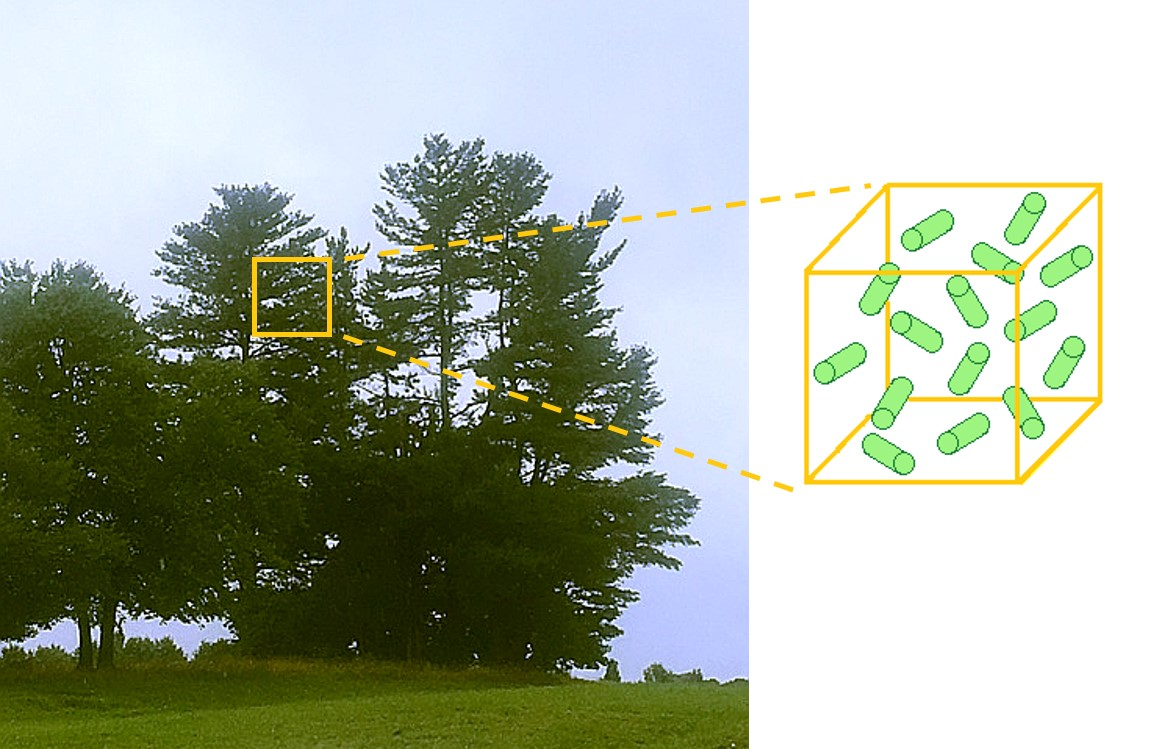
\includegraphics[width=1.0\linewidth]{Picture1.jpg}
	\caption{Vegetation translation to multi-component model}
	\label{fig:Canopymod}
\end{figure}
The force per unit volume added to the momentum equation is given by the expression:
\begin{equation}
\label{eq:DragForce}
F_{\mathrm{D}} = \frac{1}{V} \, \frac{\rho}{2} \, \sum_{i=1}^N  C_{\mathrm{D}} \, A_{\mathrm{p},i} \, {U}^2
\end{equation}
where $V$ is the volume of the grid cell, $A_{\mathrm{p},i}$ is the projected area of the $i$th vegetative component, and $C_{\mathrm{D}}$ is a drag coefficient which is taken as a constant. Similar configurations have already been been adapted in numerical investigations~\cite{Pimont2009, Dupont2008}.

Equation~(\ref{eq:DragForce}) can be recast in an equivalent form that is more useful for describing vegetation drag~\cite{Mueller2014}:
\begin{equation}
\label{eq:DragForcea}
F_{\mathrm{D}}  = \frac{\rho}{2} C_{\mathrm{D}} \, C_{\mathrm{s}} \, \beta \, \sigma \, U^2
\end{equation}
where $C_{\mathrm{s}}$ is a characteristic shape factor defined in this case as the ratio of the projected area to surface area of each vegetative component, $\beta$ is the ratio of the volume occupied by vegetation to the control volume, $V$, and $\sigma$ is the surface area to volume ratio of each vegetative component. Some of the terms are difficult to measure, such as the shape factor and surface to volume ratio. However, these terms may be combined to form a parameter that resembles an absorption coefficient ($\kappa$):
\begin{equation}
\label{eq:Kappa}
\kappa = C_{\mathrm{s}} \, \beta \, \sigma
\end{equation}
that can be determined by measuring the projected area of light passing a distance $L$ through the vegetation. The relative area of light, or ``free area fraction'', is defined by the relation:
\begin{equation}\label{eq:WhiteFraction}
W = {\rm e}^{-\kappa L}
\end{equation}
In the experiments, the cross-section of a small wind tunnel is filled with various amounts and types of vegetation to determine the drag coefficient for the following simplified model:
\begin{equation}\label{eq:Pressure}
F_{\mathrm{D}} \equiv \frac{\Delta P}{L}  = \frac{\rho}{2} \, C_{\mathrm{D}} \, \kappa \, U^2
\end{equation}



\section{Description of Experiments}
\label{sec:Experiments}
\subsection{Vegetation Preparation and Investigation Procedure}
\label{ssec:headingscap}

The vegetation chosen for this work was a Bakers Blue Spruce ({\em Picea pungens `Bakeri'}), an Evergreen Distylium (Distylium 'PIIDIST-I' Plant Patent \#24410), a Gold Rider Leyland Cypress ({\em Cupressocyparis leylandii `Gold Rider'}), a Kimberly Queen Fern ({\em Nephrolepis obliterata `Kimberly Queen'}), a Blue Shag Eastern White Pine ({\em Pinus strobus `Blue Shag'}), and a Robin Red Holly ({\em Ilex opaca}). Each sample was chosen based on its local availability. Leaf shapes were varied, including needle, elliptic, scale, and ovate.

The plant samples were cut into 0.5~\si{m} by 0.5~\si{m} by 0.5~\si{m} cubes using a simple guiding frame  (Fig.~\ref{fig:Sampleprep}). The samples completely filled the cross section of the wind tunnel forcing the flow to move through the vegetation as opposed to around it. To easily distinguish the front, back, left, and right side of the cube-shaped vegetation, each side was designated position A (PA), position B (PB), position C (PC), or position D (PD) (Fig.~\ref{fig:Vegpos}). After its initial cut, image analysis, wind tunnel measurements, and water displacement testing were conducted in subsequent order. In some cases, additional cuts were made to certain samples at the conclusion of the experimental procedure (Fig.~\ref{fig:flowchart}). The decision to make additional cuts made to the vegetation samples mainly depended on the health of the plant after an iteration in the experimental procedure. In the case of the Bakers Blue Spruce, Gold Rider Leyland Cypress, and Robin Red Holly, four iterative cuts were made with the final cut being the removal of all leaves from the vegetation.

\begin{figure} [!]
	\centering 	
	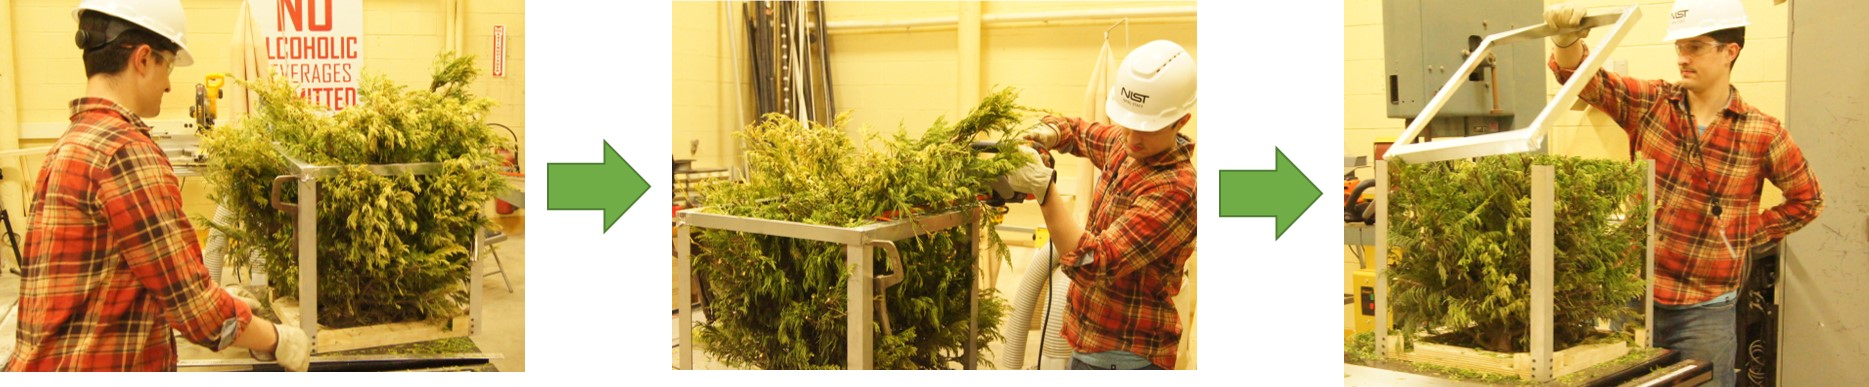
\includegraphics[height=8.in,keepaspectratio]{Picture2.jpg}
	\caption{Cutting procedure of vegetation samples}
	\label{fig:Sampleprep}
\end{figure}
\begin{figure} [!]
	\centering 	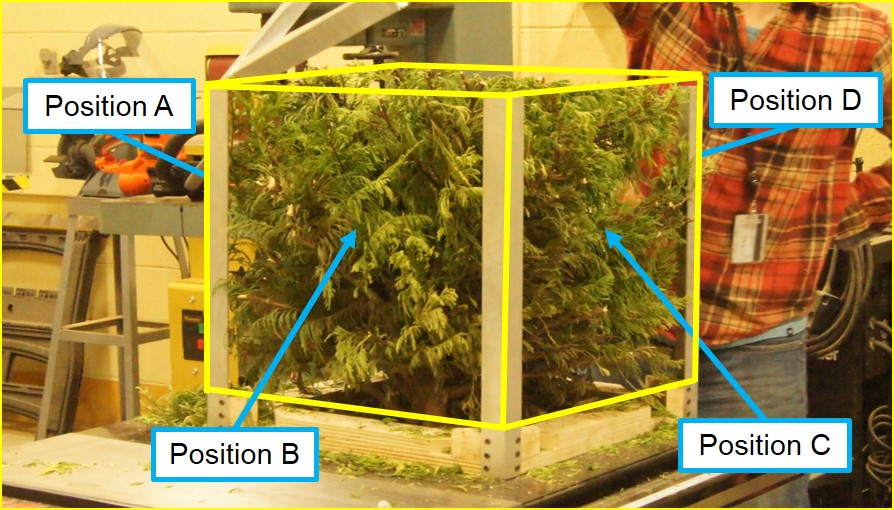
\includegraphics[width=1.0\linewidth]{Picture3.jpg}
	\caption{Prepared vegetation sample's designated orientation}
	\label{fig:Vegpos}
\end{figure}

\subsection{Image Analysis to Determine the Absorption Coefficient }
\label{ssec:headingscap}

The absorption coefficient of the vegetation samples were determined from the free area fraction ($W$) of the projected area of the sample. To determine this, the sample was placed on a table located between a large white backdrop and a 0.5~m by 0.5~m cardboard frame (Fig.~\ref{fig:ImgAnaly}), the same dimensions as the wind tunnel, providing an accurate representation of the vegetation's projected area when placed within the tunnel. For each sample cut, the projected area was photographed. All images were captured using a Nikon D5600 camera placed on a tripod located approximately 3.6~\si{m} away from the frontal plane of the vegetation sample. In order to identify smaller areas of white space, the white backdrop was illuminated using a collection of incandescent and LED lights.

\begin{figure} [!h]
	\centering 	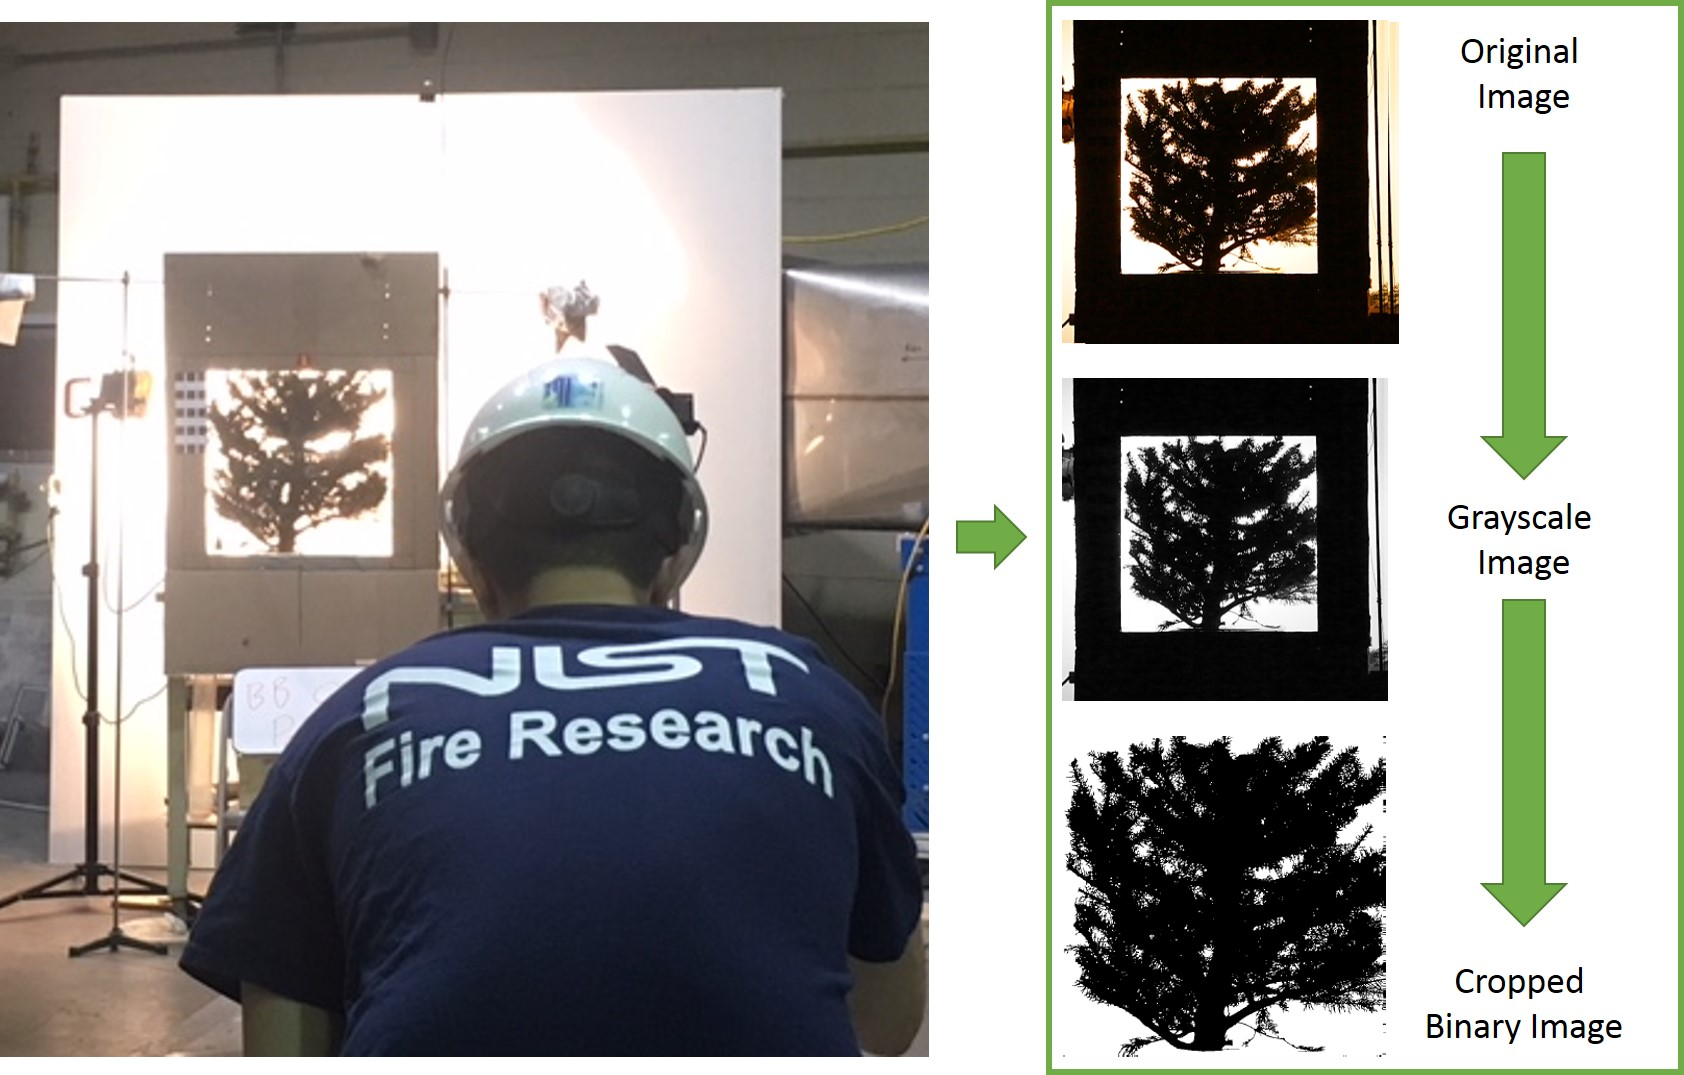
\includegraphics[width=1.0\linewidth]{Picture5.jpg}
	\caption{Setup for photographing vegetation samples (left) and the post-processing procedure for analyzing images (right)}
	\label{fig:ImgAnaly}
\end{figure}

The images were processed using MATLAB's Image Processing Toolbox. Imported images were first cropped within the cardboard frame to eliminate non-vegetative substances and to exclusively evaluate the projected vegetation area. The colored image was converted into a grey scale and then a binary (black and white) image using a pre-set threshold level. Once converted into a binary image, a pixel count was conducted to determine the free area fraction of the vegetation. After obtaining the free area fractions for each position of the vegetation sample, the average free area fraction was calculated by averaging the parallel sides of the cubic vegetation.

An uncertainty analysis was conducted by measuring objects of known projected areas using the same imaging process. It was found that with each object, the calculated free area fraction varied from the true value by 1~\%.

\subsection{Wind Tunnel Experiments to Measure the Pressure Loss Across Vegetation}
\label{ssec:headingscap}

Pressure loss measurements were obtained in a wind tunnel test section with a cross-sectional area of 0.5~\si{m} by 0.5~\si{m} and a length of 2~\si{m} Fig.~\ref{fig:WindtunnelPic}. A schematic diagram is shown in Fig.~\ref{fig:WindtunnelSch}. The volume flow through the tunnel was measured upstream of the vegetation using a Rosemont 485 Annubar. The pressure drop across the vegetation was measured using an MKS Baratron Type 220D pressure transducer with a range of 0 to 133~Pa (1~torr). The air flow was provided by a 0.91~m axial fan controlled by a variable frequency drive and monitored using the Annubar. Air density was calculated from the tunnel's internal temperature measured with a type-K thermocouple. Each sample configuration was subjected to nine different fan speeds ranging from 0 to 88~\% of the full scale fan speed. The fan speed was not run at full scale due to the risk of exceeding the pressure transducer's pressure limitations. Data was sampled at 90~\si{Hz} for a 30~\si{s} period while maintaining at a constant fan speed.

\begin{figure} [!ht]
	\centering 	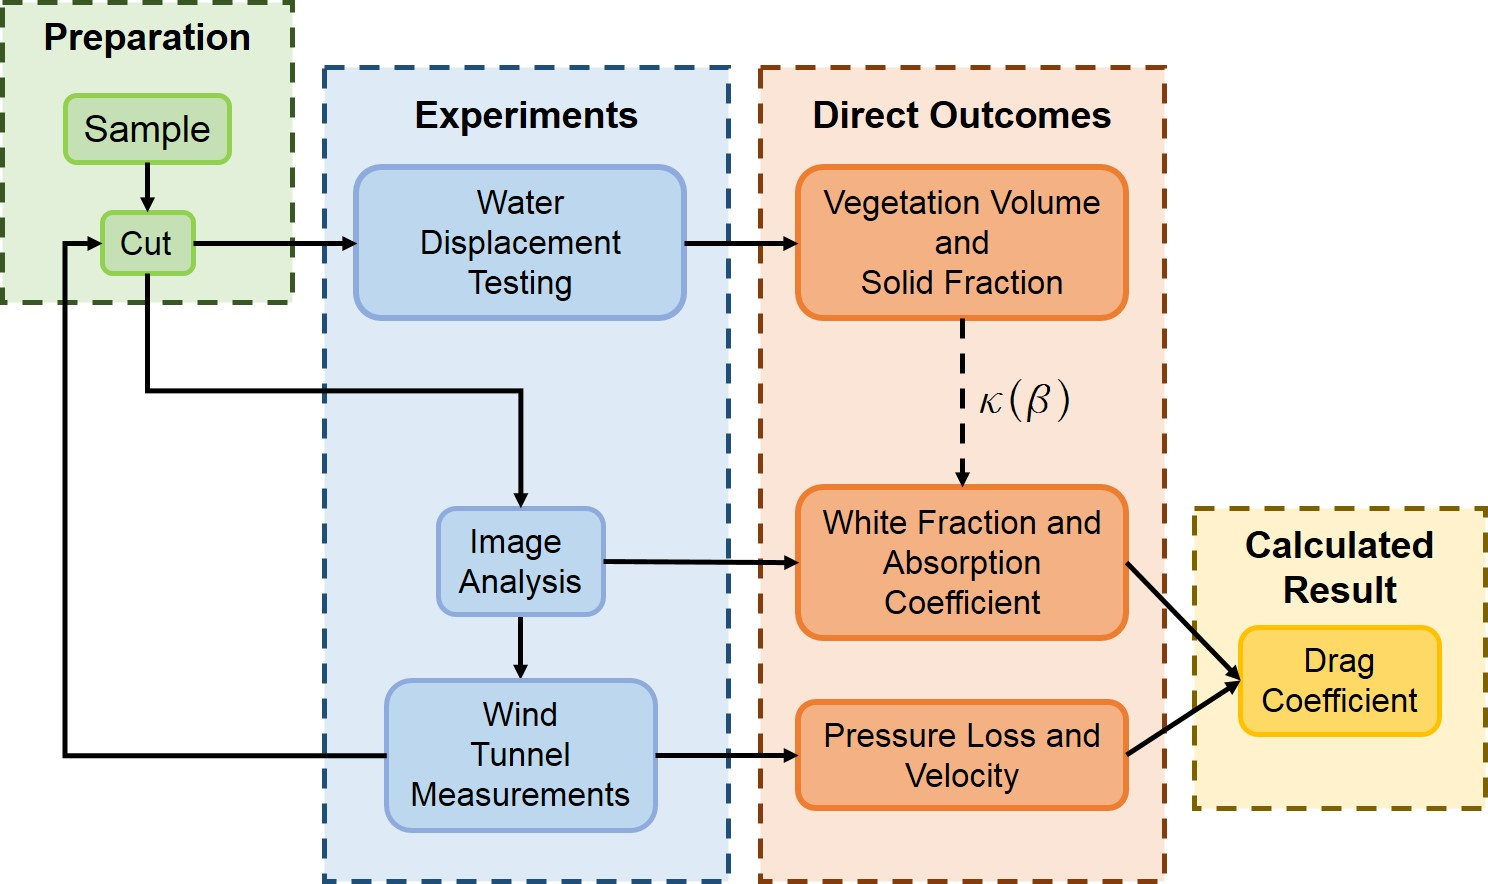
\includegraphics[width=1.0\linewidth]{Picture4.jpg}
	\caption{Wind Tunnel Experiment Setup}
	\label{fig:WindtunnelPic}
\end{figure}

\begin{figure} [!]
	\centering 	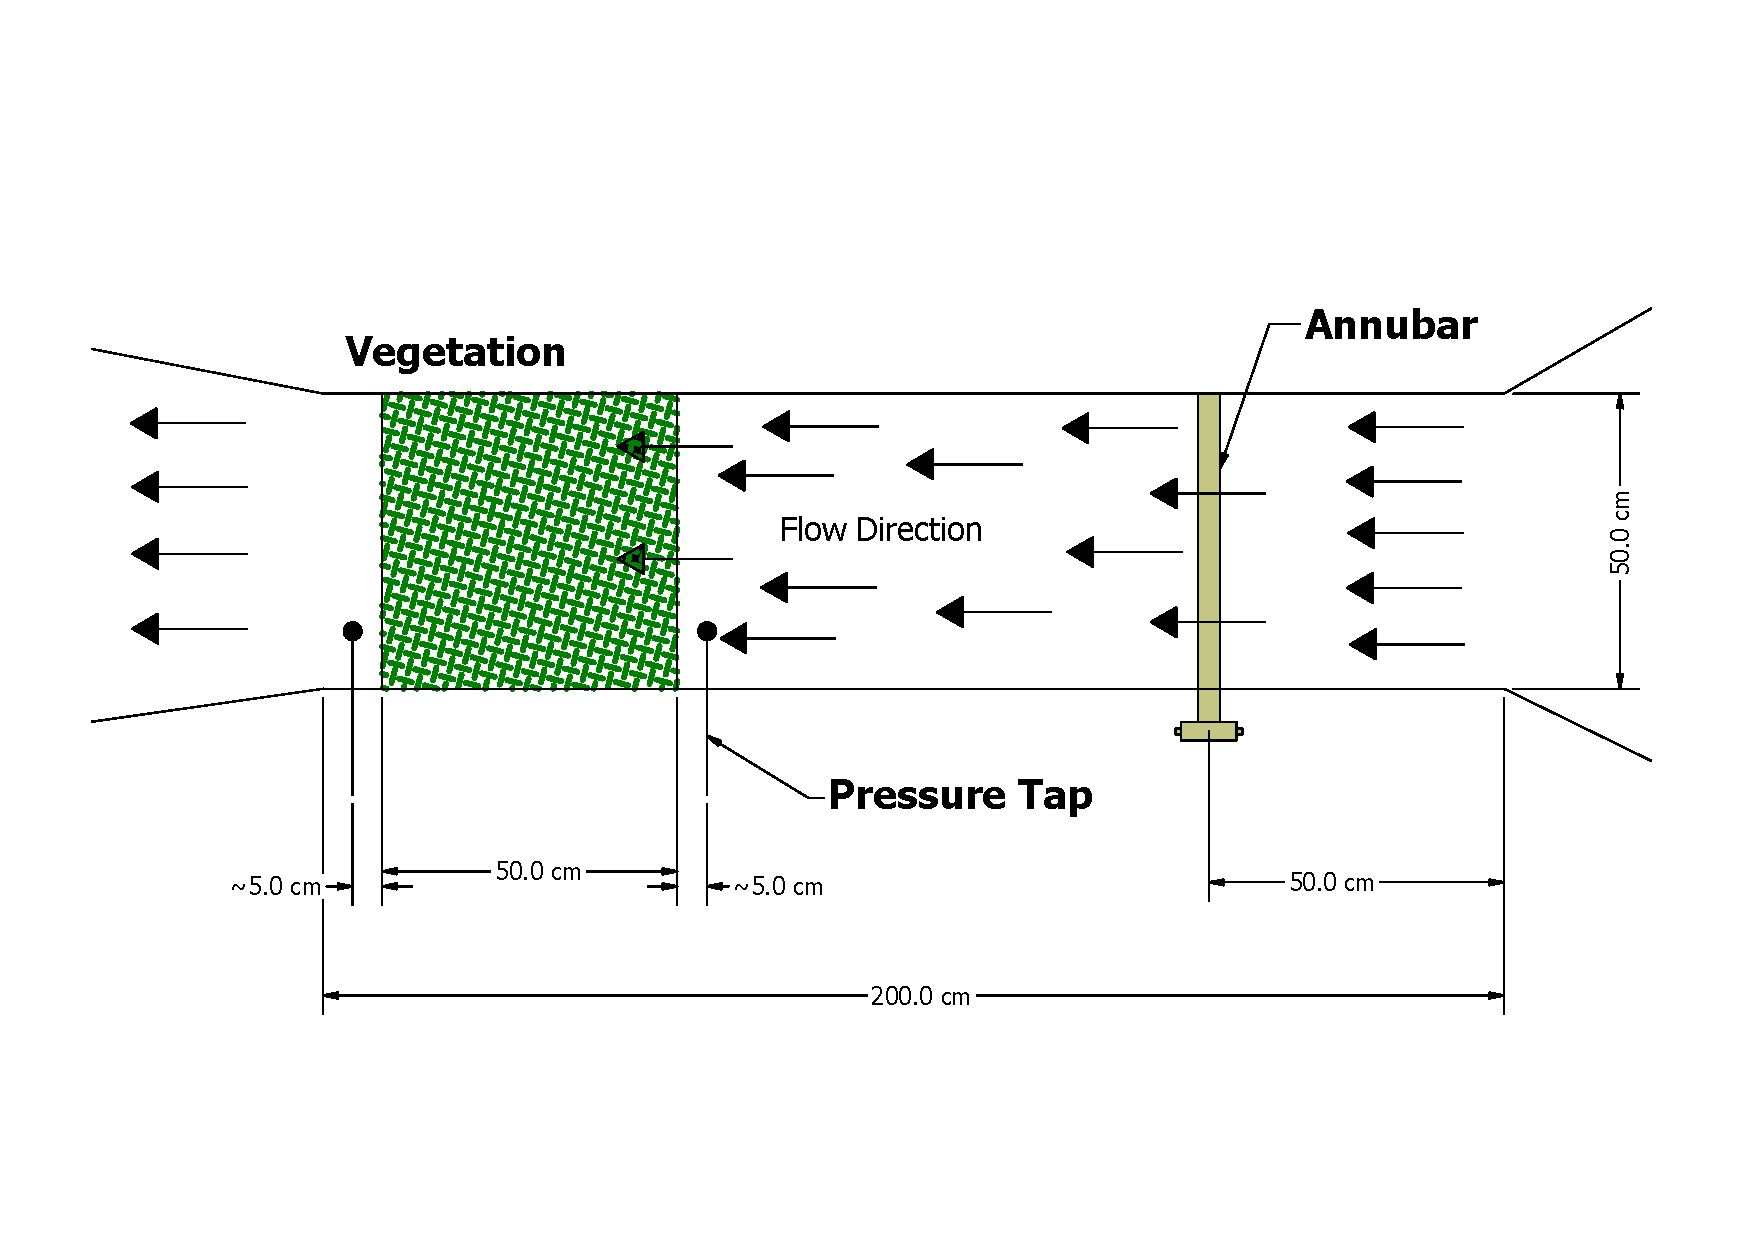
\includegraphics[width=\textwidth,keepaspectratio]{Drawing1.pdf}
	\caption{Schematic diagram of the wind-tunnel experimental setup}
	\label{fig:WindtunnelSch}
\end{figure}

Once a set of measurements were taken at all fan speeds, the wind tunnel was shut off for approximately 5~\si{min}, and then the measurements were repeated. All measurements were repeated three times for each vegetation configuration. The replicate measurements were compared using Hartley's F\textsubscript{max} test. If it was found that the data sets were homogenous, then the measurements were averaged.

The uncertainty of the pressure readings accounted for the measurement variability of the pooled data, the calibration error (1.2~\%), and the reported accuracy error (0.15~\% of the reading $\pm$ 0.02~\% of the reading per \textdegree C). Air density uncertainty was determined from the variability of the pooled data. Velocity uncertainty was established through the propagation of error incorporating the pressure and air density uncertainties. Similarly, the drag coefficient uncertainty was resolved through the propagation of error that accounted for the absorption factor uncertainty in addition to the pressure and air density uncertainty.


\subsection{Water Displacement Testing to Determine the Volume and Solid Fraction ($\beta$)}
\label{ssec:headingscap}

The volume of vegetation was measured following a cut to the vegetation sample. The vegetation was separated into two groups of branches and leaves which were packaged using a cloth mesh bag and thin wire. The volume and mass of the mesh bag and wire were pre-determined and subtracted from the total measured volume to determine the volume the vegetative solid. Before submerging the packaged material, the dry weight of the sample was measured using a Mettler Toledo Jaguar load cell. Before submerging the packaged vegetative solid, the water level was constrained to the bottom lip of a spout located approximately 3.8~\si{cm} from the top of the bucket. When the packaged vegetation was submerged, the displaced water was fed through the spout and into a glass beaker (Fig.~\ref{fig:wdt}). After the water flow through the spout of the bucket subsided, the volume of displaced water measured in a 1000 ml graduated cylinder to determine the volume of vegetation. Water displacement testing was conducted three times for each vegetation configuration. The weight of the vegetation was measured in between the displacement tests to account for any additional water that remained after the previous test. Once completing the Water Displacement Test, the solid fraction of the vegetation was calculated by dividing the average vegetation volume by the pre-determined occupied space of the vegetation (0.5~\si{m} x 0.5~\si{m} x 0.5~\si{m} = 0.125~\si{m^{3}}). The uncertainty of the vegetation volume and its respective solid fraction were determined from a combination of the variability of the repeated measurements as well as the resolution of the Mettler Toledo load cell (0.005~\si{kg}).
\begin{figure} [!]
	\centering 	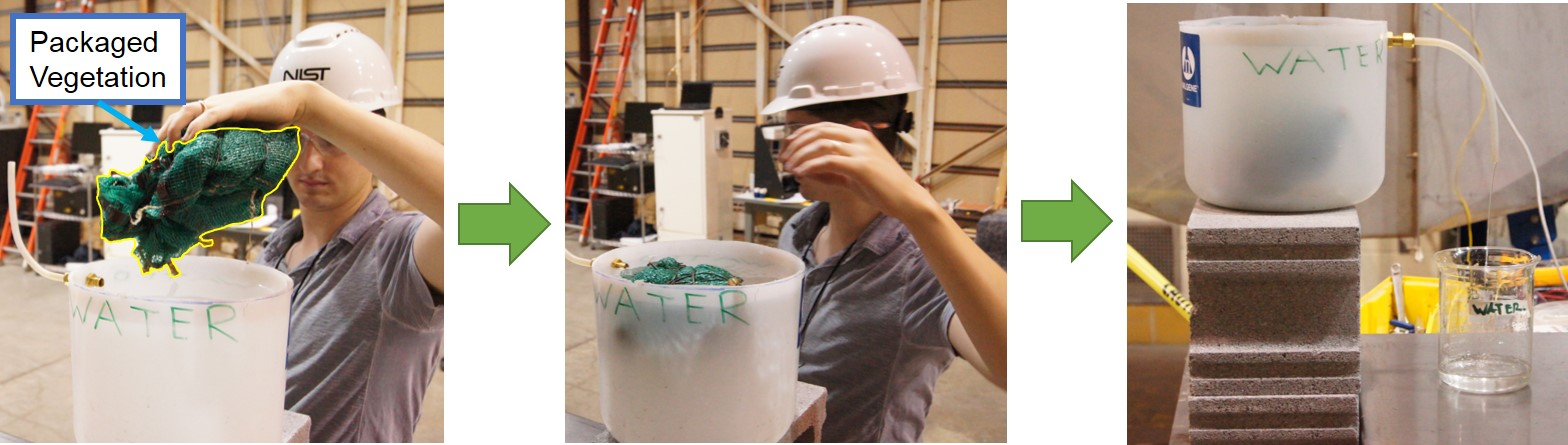
\includegraphics[height=\textheight,keepaspectratio]{Picture7.jpg}
	\caption{Procedure of the water displacement test}
	\label{fig:wdt}
\end{figure}

\pagebreak


%%%% Results section
\section{Results}
\label{sec:results}
The key results of this work is the relationship between the absorption coefficient and solid fraction and more importantly the drag coefficient derived from the measurements made in the Image Analysis and Wind Tunnel Experiments.

\subsection{Relationship between the absorption coefficient $\kappa$ and solid fraction $\beta$ }

Figure~\ref{fig:betavkappa} presents the relationship between the absorption coefficient and solid fraction of all sample configurations. The markers indicate the measured values while the dotted lines represent a linear regression fit. The linear regression fittings suggest that the absorption coefficient declines with a decrease in the solid fraction. The reduction in the solid fraction corresponds to a cut made on the vegetation sample indicating that the removal of solid material from the vegetation sample modifies the projected open area of the canopy, thus decreasing the absorption coefficient. The strong relationship between the absorption coefficient and the solid fraction demonstrated by high the coefficients of determination ($r^2$) support the formation of the absorption coefficient parameter (Eq.~\ref{eq:Kappa}). However, it should also be noted that the linear regression fittings presented in Fig.~\ref{fig:betavkappa} does not account for the fluctuating surface to volume ratio ($\sigma$) of the sample configuration, which also contributes to the $\kappa$ parameter.

\begin{sidewaysfigure}[!]
	\centering 	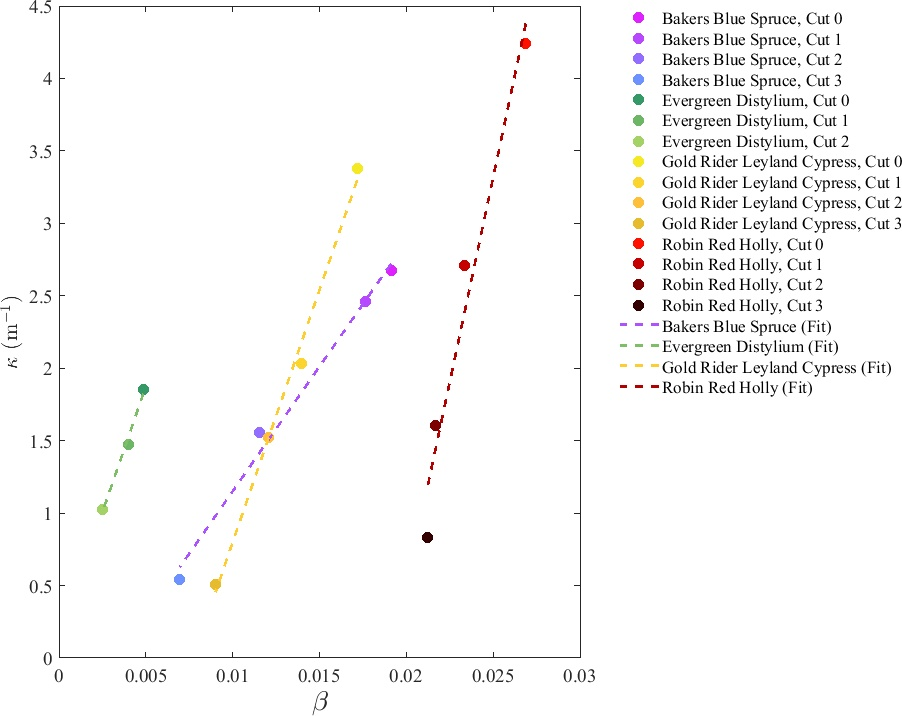
\includegraphics[width=1.1\linewidth]{Picture12.jpg}
	\caption{Calculated absorption coefficients ($\kappa$) of vegetation sample configuration plotted against their corresponding solid fractions ($\beta$) } Fig.~\ref{fig:DPoveraf(Overall)}
	\label{fig:betavkappa}
\end{sidewaysfigure}

\pagebreak


\subsection{Vegetation Canopy Drag Coefficients}
\label{ssec:headingscap}

Figure~\ref{fig:DPvU(Overall)} displays the free stream velocity for each sample configuration and the resulting differential pressure measurement is taken across the vegetation. The results of each sample configuration show that the differential pressure measured across the vegetation increases with an increase in the air velocity.  Early cuts of vegetation samples, previously shown in Fig.~\ref{fig:betavkappa} to exhibit high $\kappa$ values, appear to achieve higher differential pressure measurements taken across the vegetation compared to final cut sample configurations (no leaves configurations). The variation in the pressure loss across the vegetation concerning the variation in $\kappa$ suggests that as the plant structure obtains a higher open area, there are larger channels for larger volumes of air to move through. The results of this measurement follow previous work in which the resistance to air flow of vegetation was studied~\cite{Bitog2011}.

The ratio between the differential pressure across the vegetation over $\kappa L$ and the dynamic pressure exerted by the incoming air is presented in Fig.~\ref{fig:DPoveraf(Overall)}. In comparison to Figure~\ref{fig:DPvU(Overall)}, the differential pressure across the vegetation over $\kappa L$  for each sample configuration is observed to be linear with the dynamic pressure. The drag coefficients for each sample configuration was determined from the slope of a linear regression fitting of the measured data shown in Fig.~\ref{fig:DPoveraf(Overall)}. No linear regression fitting was observed to have a coefficient of determination value less than 0.98, indicating a close representation of the fitted regression line to the measured data. A summary of all sample configurations' (N=68) calculated drag coefficients and their respective uncertainties are presented in Table \ref{tab:SumTable}.

\begin{sidewaysfigure} [!]
	\centering
	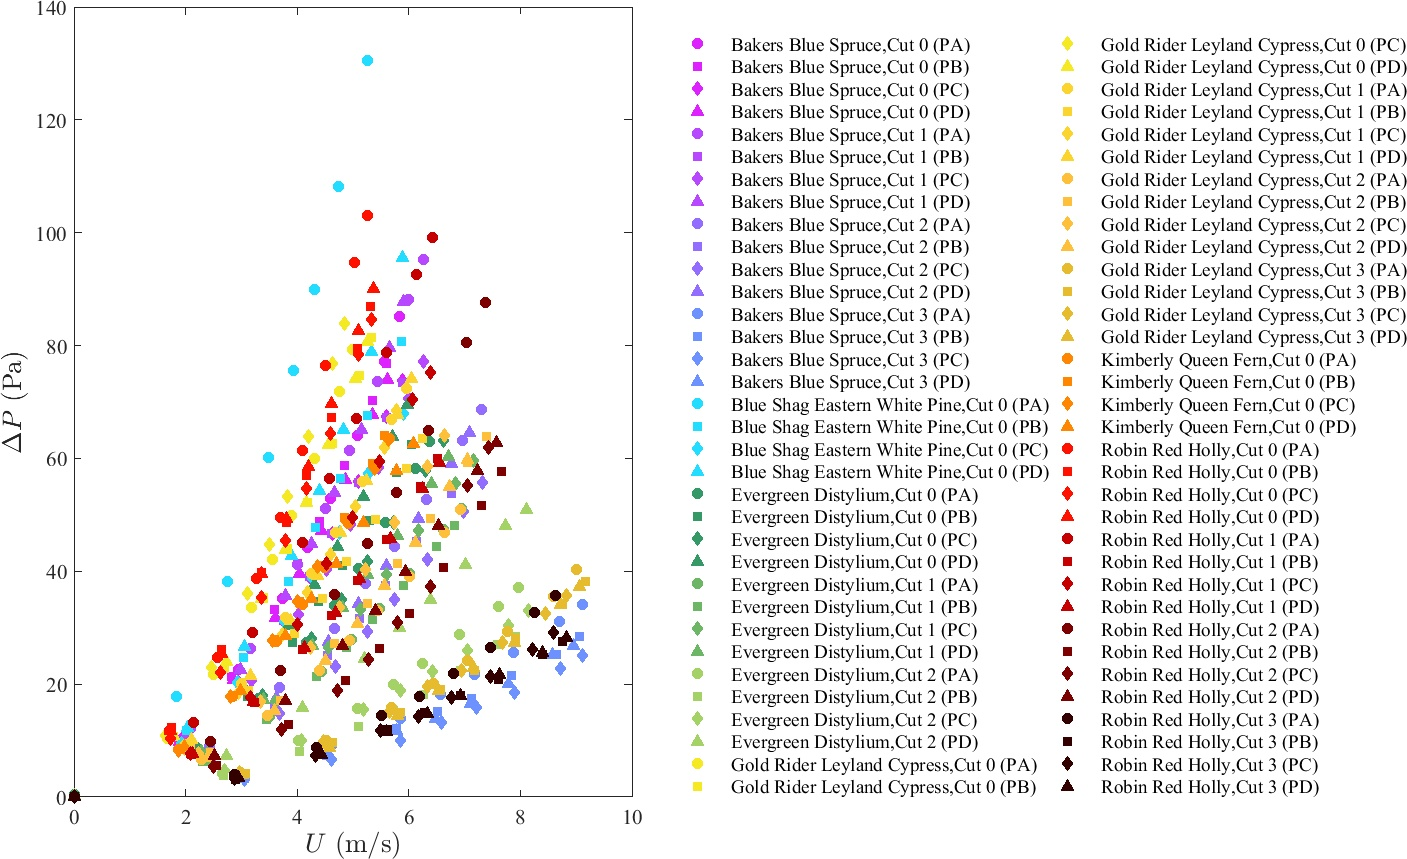
\includegraphics[width=\textwidth,keepaspectratio]{Picture8.jpg}
	\caption{Differential pressure measurements of vegetation samples subjected to a range of free stream velocities}
	\label{fig:DPvU(Overall)}
\end{sidewaysfigure}

\begin{sidewaysfigure}[!]
	\centering
	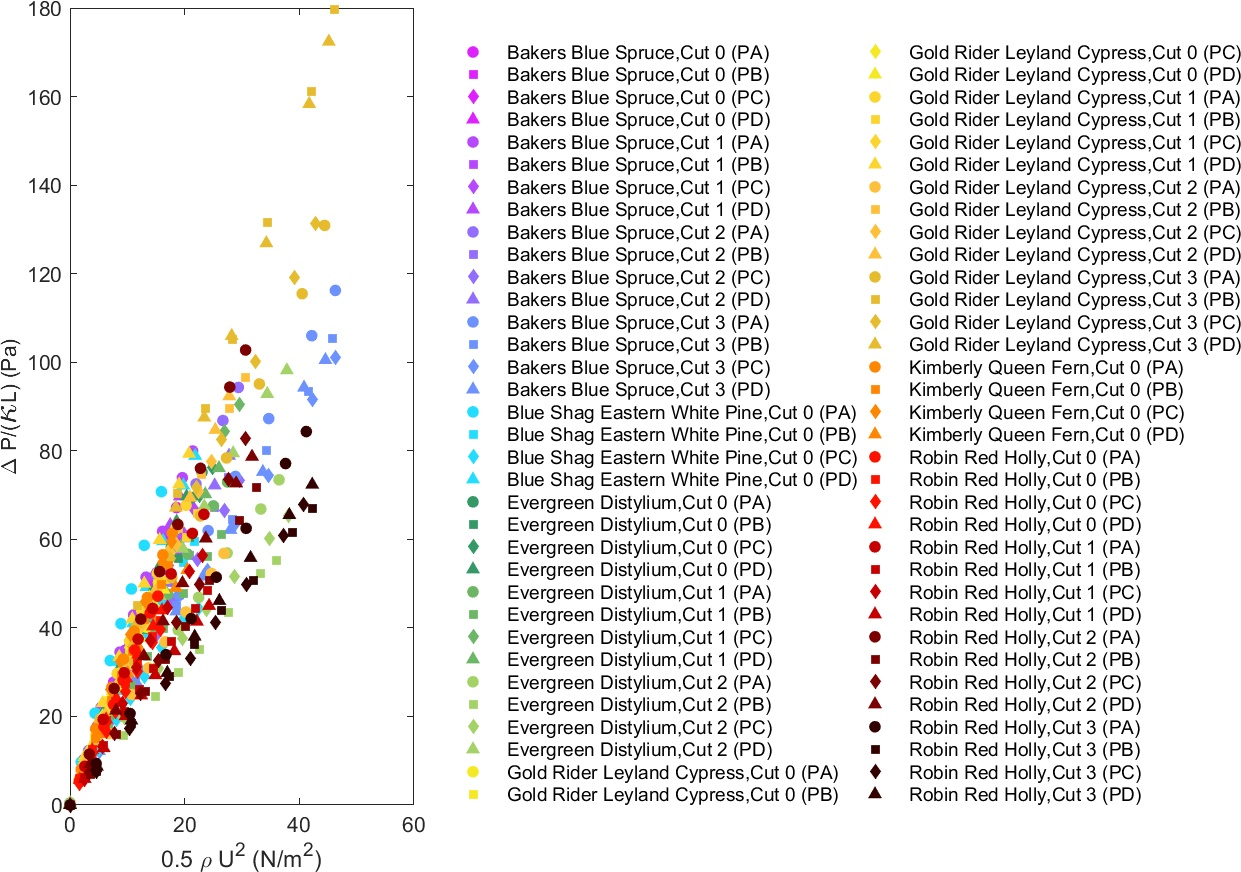
\includegraphics[width=\textwidth,keepaspectratio]{Picture9.jpg}
	\caption{Differential pressure measurements of vegetation samples over ($\kappa L$) vs. dynamic pressure}
	\label{fig:DPoveraf(Overall)}
\end{sidewaysfigure}

The distribution of all sample configurations' drag coefficient is shown in Fig.~\ref{fig:Histogram}. A Kolmogorov-Smirnov test  (K-S test) was implemented to test the normality of the drag coefficient data. The K-S test determined that the drag coefficients of all sample configurations do not significantly vary from normality, D(68)=~0.09, non-significant. The normal distribution of the data is further supported by the "bell curve" fitting displayed in  Fig.~\ref{fig:Histogram}. Additionally, the average drag coefficient of all sample configurations was determined to be 2.82 with a standard deviation of 0.62.

\begin{figure}[!h]
	%\centering 	
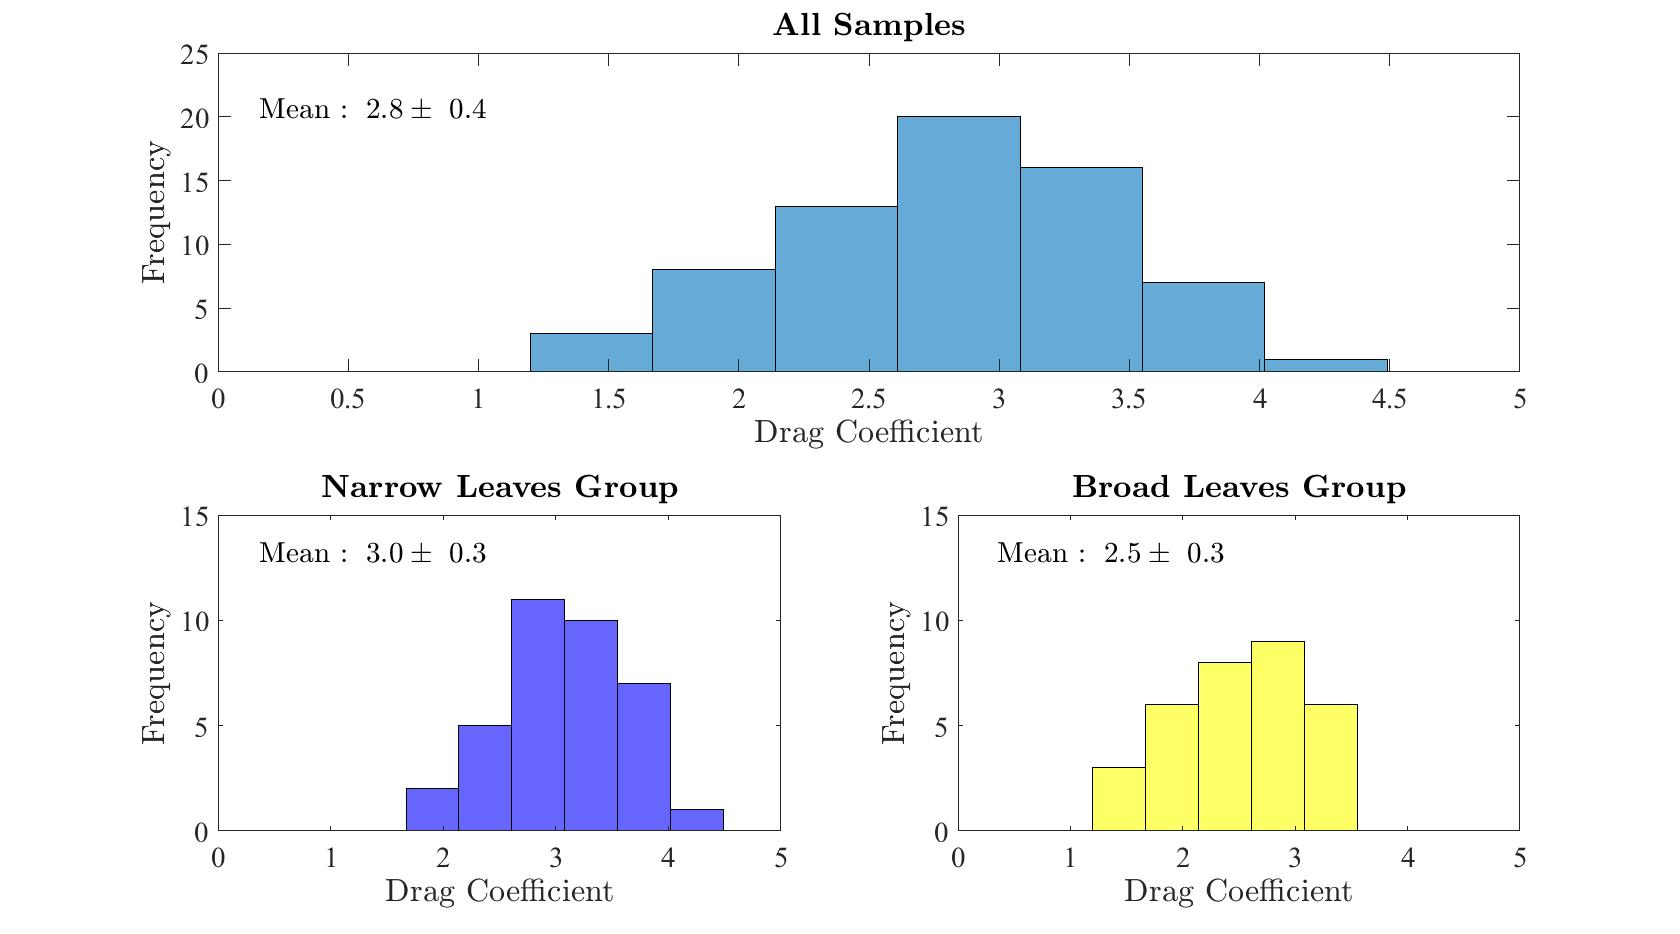
\includegraphics[width=\textwidth,keepaspectratio]{Picture11.jpg}
	\caption{Distribution of vegetation samples drag coefficients with noted mean and standard deviation values}
	\label{fig:Histogram}
\end{figure}

\begin{table}

\begin{adjustbox}{
  addcode=
    {\begin{minipage}{\width}}
    {\caption{Drag Coefficient Summary}\label{tab:SumTable}\end{minipage}},
  rotate=90,
center
}
													
	%\centering
	\footnotesize
	\begin{tabular}{cccccccccc}
	%\caption{Summary Table}	
			\hline
\textbf{Sample}		&	\textbf{Cut}	&\textbf{Position}& $C_{\rm D}$ 	&\textbf{Uncertainty}	&\textbf{Sample}	&	\textbf{Cut}	&\textbf{Position}& 	\textbf{$C_{\rm D}$ }&\textbf{Uncertainty}\\
\hline
\\[0.05cm]
Bakers Blue Spruce			&	0	&	A	& 	3.58	&	0.40				&Gold Rider Leyland Cypres&	0	&	A	& 	3.04	&	0.44	\\
					&		&	B	& 	3.15	&	0.40				&				&		&	B	& 	3.25	&	0.42	\\
					&		&	C	& 	3.11	&	0.37				&				&		&	C	& 	3.35	&	0.49	\\
					&		&	D	& 	3.04	&	0.38				&				&		&	D	& 	2.97	&	0.38	\\
					&	1	&	A	& 	3.72	&	0.37				&				&	1	&	A	& 	3.34	&	0.38	\\
					&		&	B	& 	2.98	&	0.35				&				&		&	B	& 	2.90	&	0.34	\\
					&		&	C	& 	3.07	&	0.31				&				&		&	C	& 	3.27	&	0.36	\\
					&		&	D	& 	3.60	&	0.38				&				&		&	D	& 	3.82	&	0.39	\\
					&	2	&	A	& 	3.20	&	0.30				&				&	2	&	A	& 	2.10	&	0.24	\\
					&		&	B	& 	2.65	&	0.26				&				&		&	B	& 	3.16	&	0.29	\\
					&		&	C	& 	2.47	&	0.25				&				&		&	C	& 	3.11	&	0.31	\\
					&		&	D	& 	2.83	&	0.26				&				&		&	D	& 	3.34	&	0.31	\\
					&	3	&	A	& 	2.51	&	0.34				&				&	3	&	A	& 	2.92	&	0.35	\\
					&		&	B	& 	2.26	&	0.36				&				&		&	B	& 	3.84	&	0.49	\\
					&		&	C	& 	2.16	&	0.38				&				&		&	C	& 	3.04	&	0.40	\\
					&		&	D	& 	2.25	&	0.36				&				&		&	D	& 	3.84	&	0.49	\\
					&		&		& 		&					&				&		&		& 		&		\\
Blue Shag Eastern White Pine	&	0	&	A	& 	4.02	&	0.55				&Kimberly Queen Fern	&	0	&	A	& 	3.19	&	0.38	\\
					&		&	B	& 	2.49	&	0.33				&				&		&	B	& 	2.84	&	0.35	\\	
					&		&	C	& 	1.90	&	0.29				&				&		&	C	& 	3.00	&	0.39	\\
					&		&	D	& 	3.37	&	0.38				&				&		&	D	& 	2.39	&	0.28	\\
					&		&		& 		&					&				&		&		& 		&		\\
Evergreen Distylium			&	0	&	A	& 	3.24	&	0.33				&Robin Red Holly		&	0	&	A	& 	3.08	&	0.36	\\
					&		&	B	& 	2.89	&	0.32				&				&		&	B	& 	2.60	&	0.32	\\
					&		&	C	& 	3.06	&	0.31				&				&		&	C	& 	2.50	&	0.30	\\
					&		&	D	& 	3.40	&	0.37				&				&		&	D	& 	2.72	&	0.33	\\
					&	1	&	A	& 	2.66	&	0.28				&				&	1	&	A	& 	2.81	&	0.24	\\
					&		&	B	& 	2.31	&	0.26				&				&		&	B	& 	2.00	&	0.19	\\
					&		&	C	& 	3.07	&	0.30				&				&		&	C	& 	2.53	&	0.22	\\
					&		&	D	& 	2.91	&	0.30				&				&		&	D	& 	1.83	&	0.18	\\
					&	2	&	A	& 	2.01	&	0.25				&				&	2	&	A	& 	3.36	&	0.24	\\
					&		&	B	& 	1.53	&	0.23				&				&		&	B	& 	2.20	&	0.18	\\
					&		&	C	& 	1.68	&	0.24				&				&		&	C	& 	2.66	&	0.21	\\
					&		&	D	& 	2.60	&	0.26				&				&		&	D	& 	2.48	&	0.20	\\
					&		&		& 		&					&				&	3	&	A	& 	2.05	&	0.23	\\
					&		&		& 		&					&				&		&	B	& 	1.58	&	0.22	\\
					&		&		& 		&					&				&		&	C	& 	1.64	&	0.22	\\
					&		&		& 		&					&				&		&	D	& 	1.72	&	0.23	\\
\\[0.05cm]
\hline														

	\end{tabular}
\end{adjustbox}

\end{table}

A one-way analysis of variance (ANOVA) was implemented on the drag coefficients of the different vegetation species. The analysis of the different vegetation species yielded a significant variation among the species, \textit{F}(5,62)=~4.88, \textit{p}=~7.97E-4. A Tukey HSD test subsequently applied to identify which species' average drag coefficients were significantly different from each other. The results showed one significant difference between the species' average drag coefficients: the Robin Red Holly and Gold-Rider Leyland Cypress. Despite this statistically significant difference, the average drag coefficients of the Robin Red Holly and Gold-Rider Leyland Cypress are both within one standard deviation away from the overall average drag coefficient, as demonstrated in Fig.~\ref{fig:Histogram},  and therefore is not large enough to have a practical implication. It can then be concluded that the variance of drag coefficients determined for each species is non-significant meaning the overall average drag coefficient presented in Fig.~\ref{fig:Histogram} could be applied as a consistent drag coefficient for vegetation canopies in CFD models.

\section{Comparison Between Vegetation Data and Tube Bank Models}
\label{sec:comp}

In comparison to previous work~\cite{Cao2012,Jalonen2014,Mayhead1973,Gillies2002,Ishikawa2006}, the magnitude of the measured drag coefficients in this study is relatively large. As discussed in Section~\ref{sec:intro}, most previous studies have measured the wind resistance of a single plant or tree within a larger wind tunnel while this work considered a relatively homogenous distribution of vegetation within a tunnel. The interpretation of ``free stream'' velocity, shape factor, cross sectional area, and so on, are often different in these studies, making it difficult to compare drag coefficients from one study to another. Within the field, there is no single definition of drag coefficient in regard to vegetation.

As a way to verify the accuracy of our wind tunnel measurements and the validity of our drag coefficient derivation, we considered a bank of regularly-spaced, staggered, vertical cylinders within our wind tunnel, using both actual steel rods and empirical results from Idelchick~\cite{Idelchick1994}. For each of the measured vegetation samples, a comparable configuration of vertical tubes was derived such that the volume fraction, $\beta$, free area fraction, $W$, and characteristic diameter, $D$, matched as closely as possible. The expected pressure drop through the tube bank was either measured directly in the wind tunnel or taken from Idelchick, and the corresponding drag coefficient was determined from Eq.~\ref{eq:Pressure}.

\begin{figure}[!]
	\centering 	
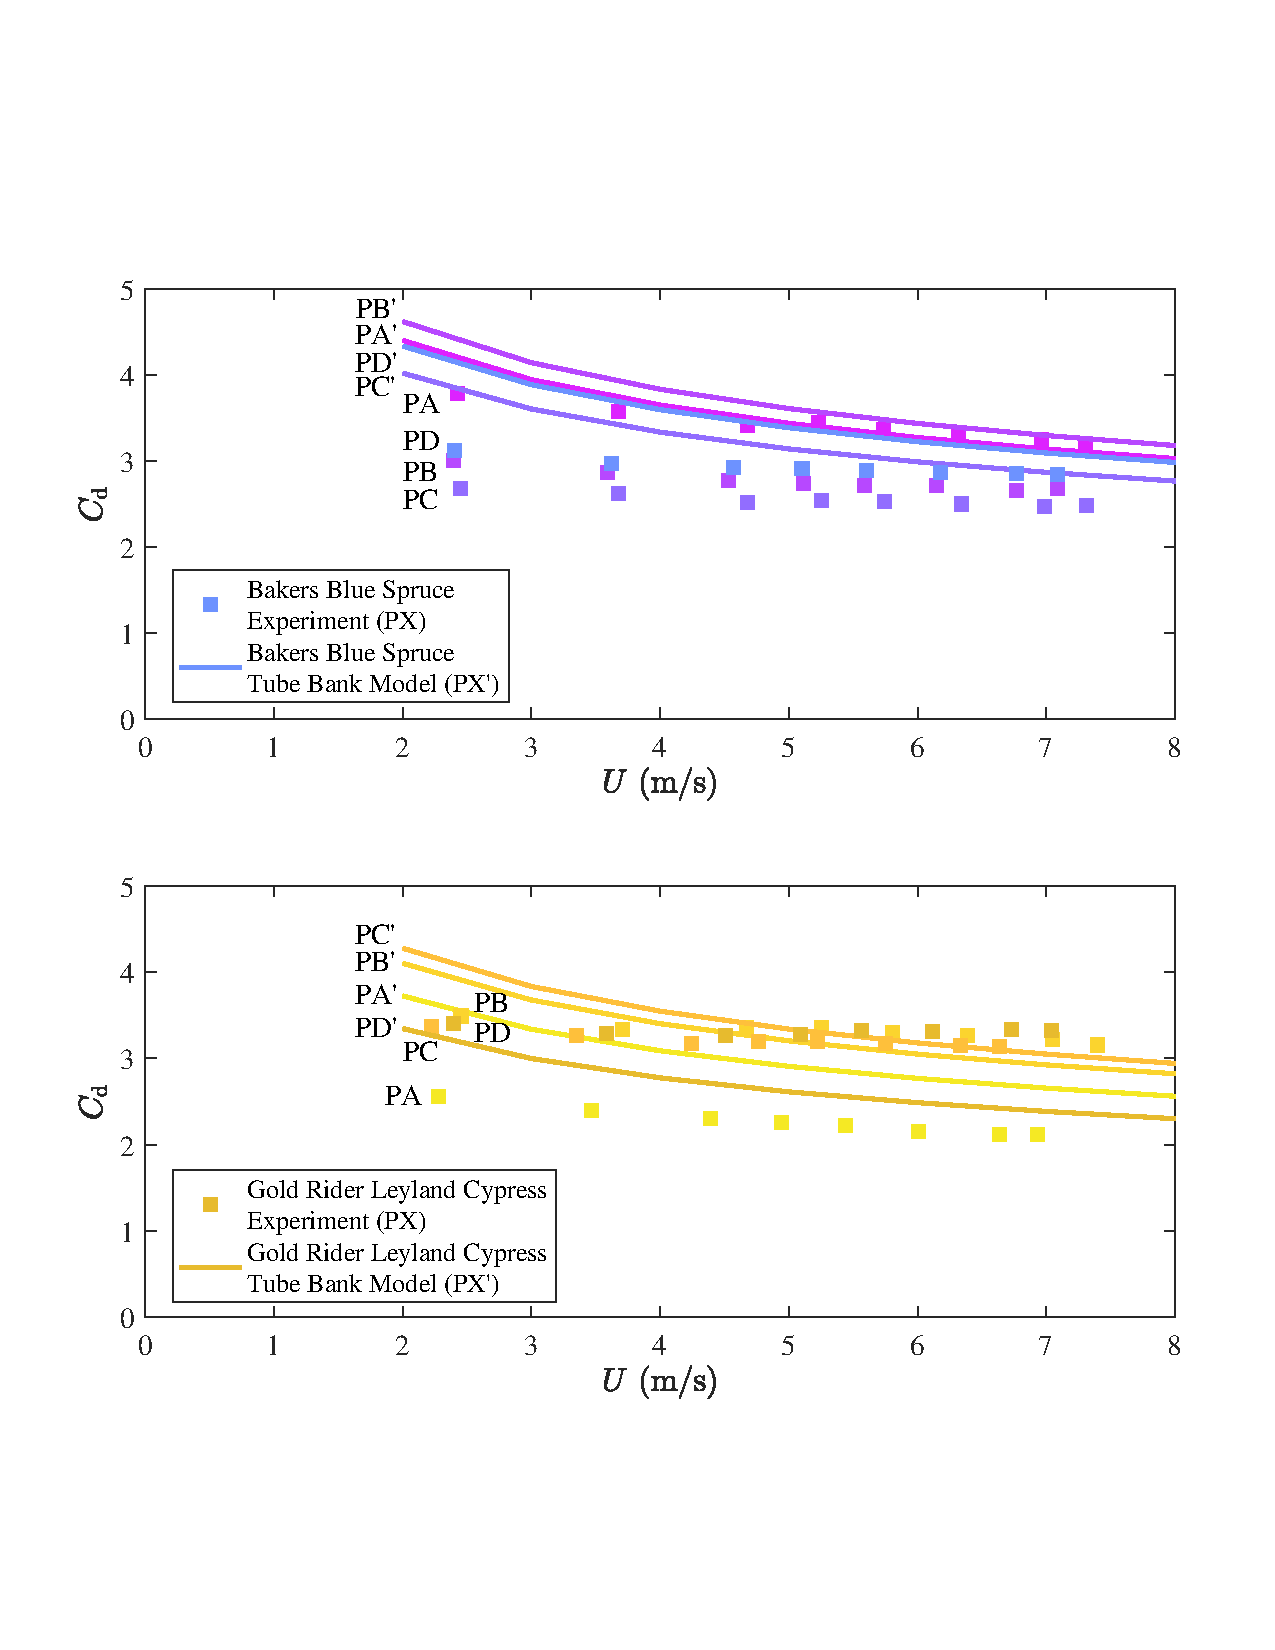
\includegraphics[width=\textwidth,keepaspectratio]{Picture13.pdf}
	\caption{Drag Coefficient comparison between Gold Rider Leyland Cypress (Cut 2) and its corresponding tube bank configuration with respect to velocity}
	\label{fig:TBGR}
\end{figure}

\begin{figure}[!]
	\centering 	
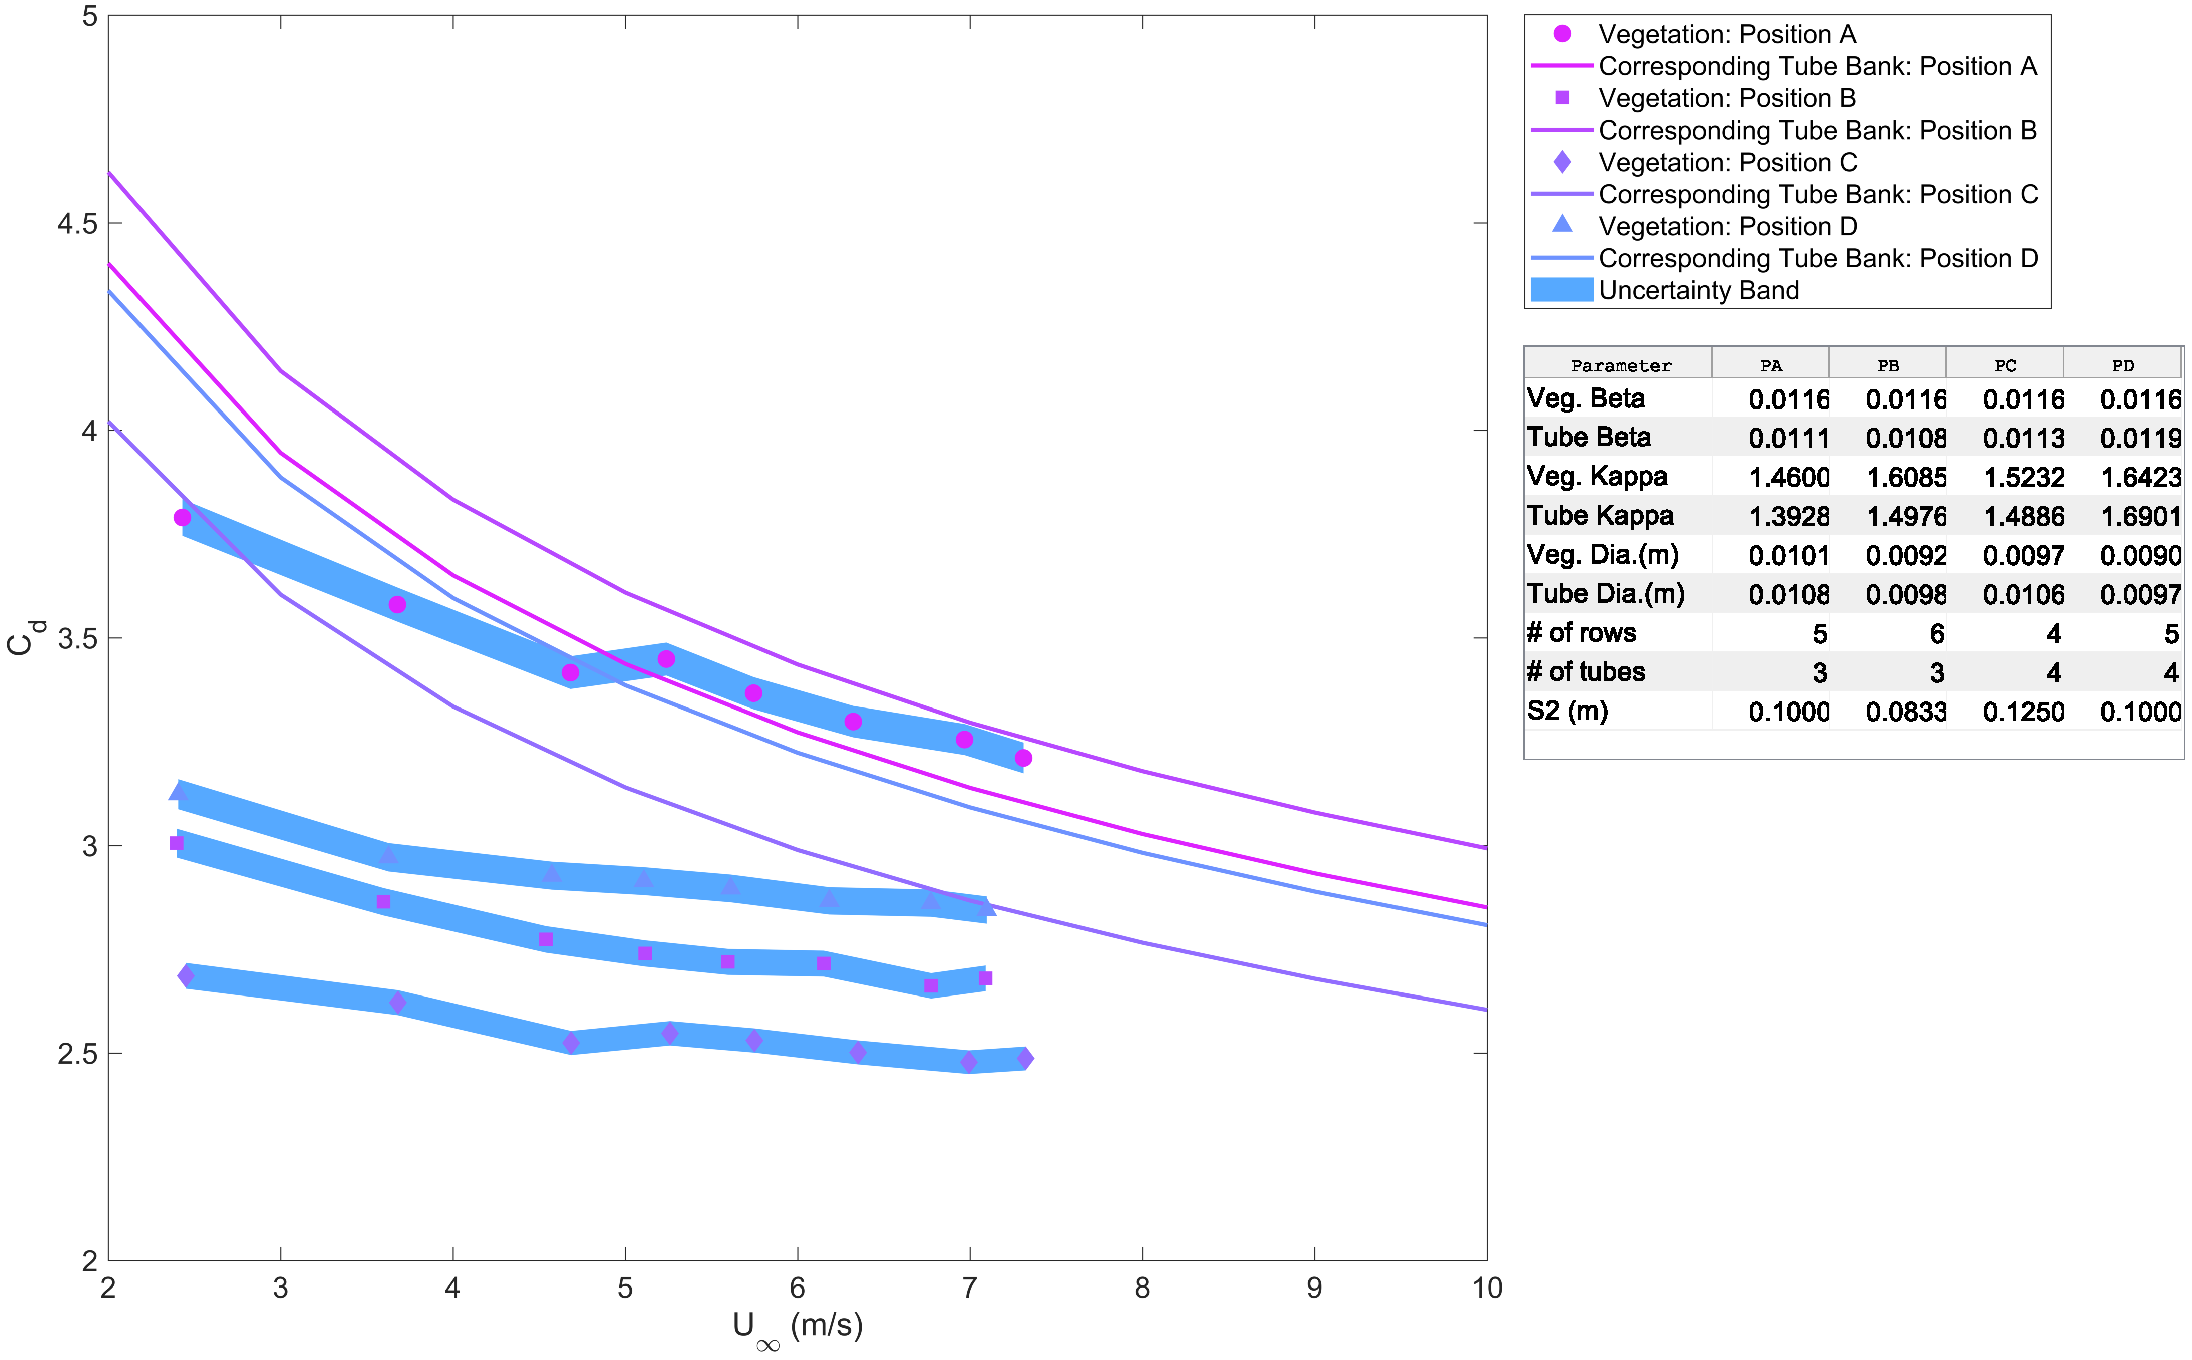
\includegraphics[width=\textwidth,keepaspectratio]{Picture14.pdf}
	\caption{Drag Coefficient comparison between Bakers Blue Spruce (Cut 2) and its corresponding tube bank configuration with respect to velocity}
	\label{fig:TBBB}
\end{figure}

Figures~\ref{fig:TBGR} and \ref{fig:TBBB} compare the drag coefficients from the Gold Rider Leyland Cypress and Bakers Blue Spruce with their tube bank equivalents. While the match is not expected to be perfect given the difference in skin fraction, shape, and so on, the drag coefficients of each configuration is comparable. 


%A hydraulic resistant tube bank model was evaluated using similar geometric features (absorption coefficient and solid fraction) of the vegetation canopy samples to compare the drag coefficients of the two different configurations.  Once a tube bank configuration was obtained, the pressure loss across the tube banks were determined using I.E. Idelchik's hydraulic resistant tube bank model.  Equation~\ref{eq:Pressure}, was then evaluated given the adjusted tube bank configuration parameters to determine the drag coefficient. It should be noted that in the calculation for the tube bank's drag coefficient, the distance L was assumed to be between rows alternative to across the entire vegetation.\\
%\indent The comparison between the vegetation sample's drag coefficient for a range of velocities and the drag coefficient of the corresponding tube bank is presented in Fig.\ref{fig:betavkappa}. It can be observed that by relatively matching the absorption coefficient, solid fraction, and average diameter of the vegetation sample, the tube bank model alligns fairly well with the measured data.


%%%%%%%%%%%%%%%%%%%%%%%%%%%%%%%%%%%%%%%%%%%%%%%%%%%%%%%%%%%%%%%%%%%%
%   Tables should appear after they are mentioned in the text.
%	Superscripted letters (a, b, c, etc.) should be used for table footnotes.
%%%%%%%%%%%%%%%%%%%%%%%%%%%%%%%%%%%%%%%%%%%%%%%%%%%%%%%%%%%%%%%%%%%%
%\begin{figure}[h]
%	\centering 	\includegraphics[width=0.5\linewidth]{Chrysanthemum.jpg}
%	\caption{This is the caption text \today}
%	\label{fig:Chrysanthemum}
%\end{figure}
%%%%%%%%%%%%%%%%%%%%%%%%%%%%%%%%%%%%%%%%%%%%%%%%%%%%%%%%%%%%%%%%%%%%
%   Figure references are “Fig. X”.
% 	“Figure X” is used at beginning of sentence.
% 	Figures should appear after they are mentioned in the text.
%	Figures must have embedded alternate text or “alt text” in order
%	to comply with Section 508 accessibility standards.
%%%%%%%%%%%%%%%%%%%%%%%%%%%%%%%%%%%%%%%%%%%%%%%%%%%%%%%%%%%%%%%%%%%%


\pagebreak

\section*{Conclusion}
This report documents a series of experiments implemented to determine the absorption coefficient, pressure loss, and the solid fraction of different types of vegetation sample configurations. The primary objective of this work was to calculate the drag coefficients of ``bulk'' vegetation that can be incorporated into CFD models. In addition to establishing drag coefficients of ``bulk''  vegetation, notable findings regarding vegetation structure and similarities between drag coefficients of plant species were also discovered from this work. It cannot be concluded, however, that the findings from this work applies to all ``bulk'' vegetation, but exclusively to the samples studied in these experiments.

\begin{enumerate}
  \item The calculated absorption coefficient for each sample demonstrated a strong relationship with its corresponding solid fraction.
  \item The overall average drag coefficient of the bulk vegetation was found to be 2.82 with a standard deviation of 0.62. The differences between the average drag coefficients of different plant species were concluded to be non-significant suggesting that the overall average drag coefficient could be used as a constant value in CFD models of various plant types.
\end{enumerate}

\section*{Acknowledgments}

\noindent Matthew Bundy and Artur Chernovksy of the National Fire Research Laboratory assisted in conducting these experiments and in processing the data.   \\
%%%%%%%%%%%%%%%%%%%%%%%%%%%%%%%%%%%%%%%%%%%%%%%%%%%%%%%%%%%%%%%%%%%%
%   Acknowledgments not required
%%%%%%%%%%%%%%%%%%%%%%%%%%%%%%%%%%%%%%%%%%%%%%%%%%%%%%%%%%%%%%%%%%%%
\pagebreak
\section*{References}
\addcontentsline{toc}{section}{References}
\bibliographystyle{techpubs}
\bibliography{References}

%%%%%%%%%%%%%%%%%%%%%%%%%%%%%%%%%%%%%%%%%%%%%%%%%%%%%%%%%%%%%%%%%%%%
%   Please use the techpubs BibTeX style when compiling bibliography, or follow the instructions on tinyurl.com/techpubsnist to format your .bib / .bbl file appropriately.
%%%%%%%%%%%%%%%%%%%%%%%%%%%%%%%%%%%%%%%%%%%%%%%%%%%%%%%%%%%%%%%%%%%%
%%%%%%%%%%%%%%%%%%%%%%%%%%%%%%%%%%%%%%%%%%%%%%%%%%%%%%%%%%%%%%%%%%%%
%   Authors who have supplemental materials should submit them when submitting their manuscripts for review. Supplemental materials may include computer code or data files associated with the paper. A brief description of the supplemental material must be included in the paper. A DOI will be assigned to the supplemental material and inserted into the paper by the Information Services Office.
%%%%%%%%%%%%%%%%%%%%%%%%%%%%%%%%%%%%%%%%%%%%%%%%%%%%%%%%%%%%%%%%%%%%

\end{document}
